\section{1. Lasso та Ridge}

\markright{Частина 1}

Регресія ласо (Lasso) та рідж-регресія (Ridge) є методами регуляризації,
які використовуються для стабілізації оцінювання параметрів.


\Needspace{167pt}

\subsection{1.а Концепція Lasso}

\begin{taskstatement}Поясніть своїми словами концепцію регресії ласо. Опишіть сценарій, за
якого звичайна лінійна регресія зазнає невдачі (наприклад, через
мультиколінеарність або коли \(p > n\)), але регресію ласо все ще можна
оцінити. Чому нам потрібно максимізувати цільову функцію чисельно (на
відміну від рідж-регресії, яка має аналітичний розв'язок)?
\end{taskstatement}

\par\medskip
Lasso додає до суми квадратів залишків штраф за суму модулів
коефіцієнтів. Штраф зменшує коефіцієнти, а частину може зробити точно
нульовими, тому Lasso одночасно виконує відбір ознак.
\[RSS+\lambda\sum_{j=1}^{p}|\beta_j|\longrightarrow\min.\] Тут \(RSS\)
позначає суму квадратів залишків, \(\lambda>0\) є силою штрафу, \(p\)
кількістю ознак, а \(\beta_j\) коефіцієнтом ознаки з номером \(j\).
Вільний член у цьому записі опущено завдяки центруванню даних.

Якщо дві ознаки дублюють одна одну або ознак більше, ніж спостережень
(\(p>n\), де \(n\) позначає кількість спостережень), матриця \(X^TX\)
вироджена і звичайна формула МНК з оберненою матрицею не працює. Тут
\(X\) позначає матрицю ознак. Мінімум RSS усе ще існує, але коефіцієнти
можуть бути неєдиними. Сильна, але неточна колінеарність робить оцінки
нестійкими. Lasso зі штрафом можна оцінити й у цих випадках, хоча при
точному дублюванні ознак його коефіцієнти теж не обов'язково єдині.

Функцію потрібно мінімізувати, а не максимізувати. Модуль не має
похідної в нулі, тому для загальної матриці ознак немає простої
матричної формули, як у Ridge. Один із чисельних методів, покоординатний
спуск, по черзі оновлює коефіцієнти до збіжності. Для спеціальних
випадків, наприклад ортогональних ознак, явний розв'язок існує.


\Needspace{422pt}

\subsection{1.б Масштабування та кодування}

\begin{taskstatement}Для звичайної регресії МНК змінні рідко нормуються. Однак у випадку
ласо-регресії масштабування є критичним, оскільки штраф накладається
безпосередньо на абсолютну величину коефіцієнтів. Чому це так?
Масштабуйте числові дані за допомогою StandardScaler. Чи можна / чи
потрібно масштабувати бінарні змінні (даммі) в такий самий спосіб? Як
обробити факторні змінні (наприклад, FireplaceQu) через OneHotEncoder?
\end{taskstatement}

\pythoncode{p1-c9}

\begingroup\fontsize{7.5}{9.5}\selectfont\setlength{\tabcolsep}{2.5mm}\renewcommand{\arraystretch}{1.12}
\begin{longtable}{|lll|}
\hline
Ознака & Середнє після заповнення & Масштаб Standard\allowbreak{}Scaler \\
\hline
\endfirsthead
\hline
Ознака & Середнє після заповнення & Масштаб Standard\allowbreak{}Scaler \\
\hline
\endhead
\hline\endfoot
Lot\allowbreak{}Frontage & 69.0051 & 21.3641 \\
Lot\allowbreak{}Area & 10127.9 & 8049.19 \\
Overall\allowbreak{}Qual & 6.06442 & 1.38822 \\
Overall\allowbreak{}Cond & 5.58191 & 1.10542 \\
Year\allowbreak{}Built & 1970.51 & 30.335 \\
Year\allowbreak{}Remod\allowbreak{}Add & 1983.92 & 20.7819 \\
Mas\allowbreak{}Vnr\allowbreak{}Area & 97.741 & 171.73 \\
Bsmt\allowbreak{}Fin\allowbreak{}SF1 & 442.503 & 452.032 \\
Bsmt\allowbreak{}Fin\allowbreak{}SF2 & 50.0759 & 170.327 \\
Bsmt\allowbreak{}Unf\allowbreak{}SF & 554.354 & 433.607 \\
Total\allowbreak{}Bsmt\allowbreak{}SF & 1047 & 436.383 \\
1st\allowbreak{}Flr\allowbreak{}SF & 1154.81 & 385.032 \\
2nd\allowbreak{}Flr\allowbreak{}SF & 333.688 & 427.05 \\
Low\allowbreak{}Qual\allowbreak{}Fin\allowbreak{}SF & 4.35708 & 44.3145 \\
Gr\allowbreak{}Liv\allowbreak{}Area & 1492.86 & 504.512 \\
Bsmt\allowbreak{}Full\allowbreak{}Bath & 0.431314 & 0.525356 \\
Bsmt\allowbreak{}Half\allowbreak{}Bath & 0.0593003 & 0.241544 \\
Full\allowbreak{}Bath & 1.55717 & 0.552044 \\
Half\allowbreak{}Bath & 0.370734 & 0.499502 \\
Bedroom\allowbreak{}Abv\allowbreak{}Gr & 2.84514 & 0.820177 \\
Kitchen\allowbreak{}Abv\allowbreak{}Gr & 1.04309 & 0.211294 \\
Tot\allowbreak{}Rms\allowbreak{}Abv\allowbreak{}Grd & 6.40913 & 1.56332 \\
Fireplaces & 0.598976 & 0.652848 \\
Garage\allowbreak{}Cars & 1.74701 & 0.746145 \\
Garage\allowbreak{}Area & 469.082 & 212.342 \\
Wood\allowbreak{}Deck\allowbreak{}SF & 94.1131 & 124.825 \\
Open\allowbreak{}Porch\allowbreak{}SF & 47.3417 & 68.0229 \\
Enclosed\allowbreak{}Porch & 24.7317 & 67.0166 \\
3Ssn\allowbreak{}Porch & 2.42278 & 24.5191 \\
Screen\allowbreak{}Porch & 16.0102 & 55.809 \\
Pool\allowbreak{}Area & 2.58276 & 38.316 \\
Misc\allowbreak{}Val & 58.055 & 623.242 \\
Mo\allowbreak{}Sold & 6.18473 & 2.70783 \\
Yr\allowbreak{}Sold & 2007.79 & 1.31484 \\
\end{longtable}
\par\nopagebreak\vspace{1pt}{\itshape\color{black!60}Скорочено: пропущено колонки «Середнє після стандартизації» (усі приблизно 0) та «SD після стандартизації» (усі дорівнюють 1).}
\endgroup


\Needspace{46.8pt}

\resulttext{p1-c9-out1.txt}

\Needspace{82pt}
\begingroup\fontsize{7.5}{9.5}\selectfont\setlength{\tabcolsep}{2.5mm}\renewcommand{\arraystretch}{1.12}\par\noindent\begin{tabular}{|ll|}
\hline
Ознака & Невідомих значень у перевірочній частині \\
\hline
Exterior2nd & 1 \\
Electrical & 1 \\
Kitchen\allowbreak{}Qual & 1 \\
Misc\allowbreak{}Feature & 1 \\
\hline
\end{tabular}
\par\endgroup


\answerheading
Якщо площу перевести у більші одиниці, її коефіцієнт має збільшитися,
щоб прогноз залишився тим самим. RSS від цього не зміниться, а штраф за
модуль коефіцієнта зросте. Тому без масштабування Lasso нерівномірно
штрафує однакові за змістом ефекти.

\texttt{StandardScaler} обчислює \(z_{ij}=(x_{ij}-\bar x_j)/s_j\), де
\(x_{ij}\) є значенням ознаки \(j\) для будинку \(i\), \(\bar x_j\) її
навчальним середнім, а \(s_j\) навчальним стандартним відхиленням із
дільником \(n\); \(z_{ij}\) є стандартизованим значенням. Після цього
числовий коефіцієнт описує зміну ціни при збільшенні ознаки на одне
навчальне стандартне відхилення. Для звичайного МНК з вільним членом
таке оборотне перетворення не змінює підгонку, хоча може покращити
числову стійкість.

Даммі теж можна стандартизувати: для частки одиниць \(q\) її стандартне
відхилення дорівнює \(\sqrt{q(1-q)}\). Це змінює відносну силу штрафу
для рідкісних і частих категорій. Єдиного обов'язкового вибору немає.
Тут залишаємо даммі у шкалі 0/1, щоб коефіцієнт відповідав переходу від
базової категорії до заданої; це свідомий вибір шкали штрафу.

\texttt{OneHotEncoder(drop="first")} створює індикатори для всіх
категорій, крім базової. Для \texttt{FireplaceQu} базовий рівень
\texttt{Ex}, а \texttt{NA} означає відсутність каміна й має окрему
даммі.

Параметри масштабування та перелік категорій визначаємо за навчальними
даними.


\Needspace{411pt}

\subsection{1.в Вибір штрафу Lasso}

\begin{taskstatement}Запустіть регресію ласо за допомогою Lasso або LassoCV з коефіцієнтом
регуляризації \(\alpha > 0\) (\(\alpha\) в sklearn відповідає
\(\lambda\) в теоретичних формулах). Побудуйте графік залежності
оцінених параметрів від \(\alpha\). Яке значення \(\alpha\) ви б
рекомендували? Визначте оптимальний \(\alpha\) за допомогою 5-блочної
крос-валідації (LassoCV).
\end{taskstatement}

\pythoncode{p1-c12}

\Needspace{56pt}
\begingroup\fontsize{7.5}{9.5}\selectfont\setlength{\tabcolsep}{2.5mm}\renewcommand{\arraystretch}{1.12}\par\noindent\begin{tabular}{|lll|}
\hline
Метод & alpha & CV MSE, дол.\textasciicircum{}2 \\
\hline
Lasso\allowbreak{}CV: спільна підготовка & 76.2699 & 9.81199e+08 \\
Pipeline: підготовка в кожному блоці & 76.2699 & 9.82068e+08 \\
\hline
\end{tabular}
\par\endgroup


\Needspace{37.599999999999994pt}

\resulttext{p1-c12-out1.txt}

\begin{figure}[H]\centering
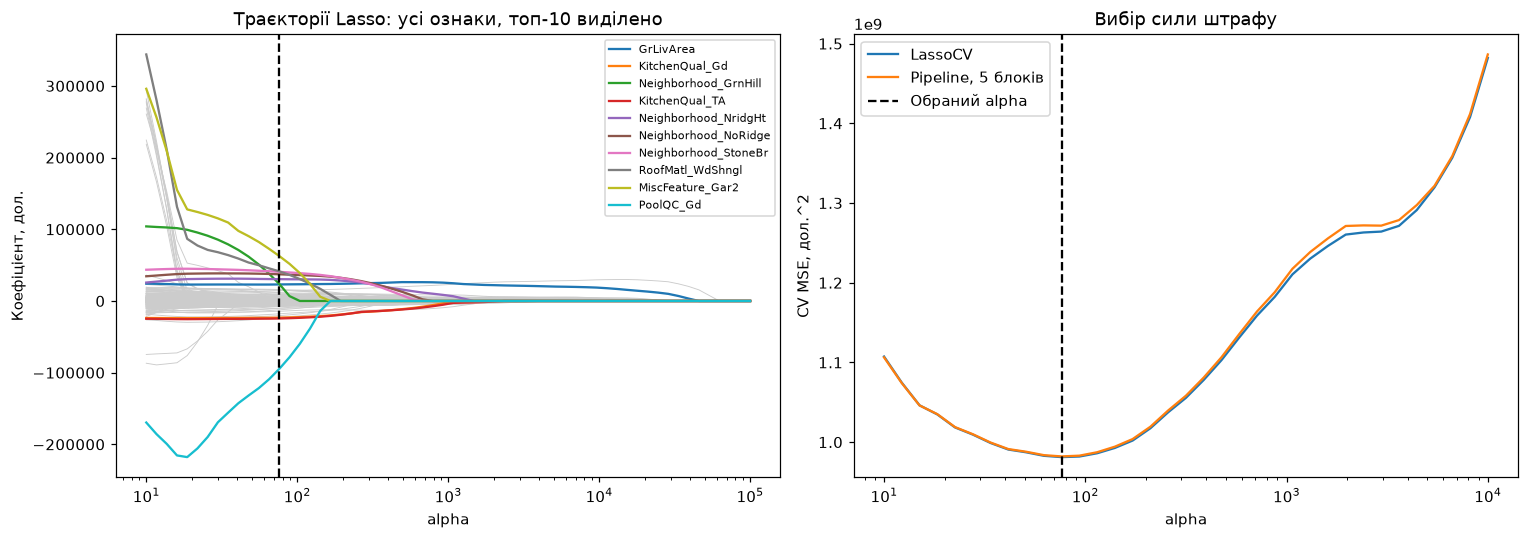
\includegraphics[width=1\linewidth,height=0.85\textheight,keepaspectratio]{../../figures/part1_lasso.png}
\caption{Траєкторії коефіцієнтів і вибір штрафу Lasso.}
\end{figure}

\Needspace{290pt}
\begingroup\fontsize{7.5}{9.5}\selectfont\setlength{\tabcolsep}{2.5mm}\renewcommand{\arraystretch}{1.12}\par\noindent\begin{tabular}{|ll|}
\hline
 & Коефіцієнт Lasso \\
\hline
Pool\allowbreak{}QC\_Gd & -94452.8 \\
Misc\allowbreak{}Feature\_Gar2 & 62519.3 \\
Roof\allowbreak{}Matl\_Wd\allowbreak{}Shngl & 41280.6 \\
Neighbor\-hood\_Stone\allowbreak{}Br & 40662.6 \\
Neighbor\-hood\_No\allowbreak{}Ridge & 37231.7 \\
Neighbor\-hood\_Nridg\allowbreak{}Ht & 30428.6 \\
Kitchen\allowbreak{}Qual\_TA & -24421.7 \\
Neighbor\-hood\_Grn\allowbreak{}Hill & 23490.9 \\
Kitchen\allowbreak{}Qual\_Gd & -23299.2 \\
Gr\allowbreak{}Liv\allowbreak{}Area & 23057.6 \\
Bldg\allowbreak{}Type\_Twnhs & -22854.1 \\
Kitchen\allowbreak{}Qual\_Fa & -20387.4 \\
Bldg\allowbreak{}Type\_Twnhs\allowbreak{}E & -17866 \\
Land\allowbreak{}Contour\_HLS & 15980.7 \\
Neighbor\-hood\_Somerst & 15094.3 \\
Exterior1st\_Brk\allowbreak{}Face & 15034.8 \\
Bsmt\allowbreak{}Qual\_Gd & -14333.7 \\
Overall\allowbreak{}Qual & 14157.1 \\
Lot\allowbreak{}Shape\_IR3 & -12279 \\
Condition1\_Pos\allowbreak{}N & 11470.3 \\
\hline
\end{tabular}
\par\nopagebreak\vspace{1pt}{\itshape\color{black!60}Скорочено: із 126 ненульових коефіцієнтів Lasso показано 20 найбільших за модулем.}
\par\endgroup


\answerheading
Середня квадратична помилка прогнозу визначається як
\(MSE=\frac{1}{m}\sum_{i=1}^{m}(y_i-\widehat y_i)^2\), де \(m\) є
кількістю перевірочних спостережень, \(y_i\) фактичною ціною, а
\(\widehat y_i\) прогнозом для будинку \(i\). Одиниці MSE тут дол.². Для
крос-валідації обчислюємо цю помилку окремо на кожному відкладеному
блоці.

Для кожного штрафу навчаємо модель на чотирьох блоках і прогнозуємо
п'ятий. Вибираємо мінімум
\(CV(\alpha)=\frac15\sum_{k=1}^{5}MSE_k(\alpha)\), де \(MSE_k\) є
середньою квадратичною помилкою на відкладеному блоці \(k\). Це найкраще
значення серед перевіреної сітки, а не доведений мінімум серед усіх
додатних чисел.

\texttt{LassoCV} виконує вимогу завдання, але отримує вже масштабовану
матрицю: середні та медіани тоді використовують усю навчальну частину,
включно з внутрішніми перевірочними блоками. Тому додатково застосовано
\texttt{GridSearchCV} до повного \texttt{Pipeline}, де підготовка
відбувається окремо в кожному блоці. Для фінальної моделі рекомендую
штраф із цього другого порівняння; конкретні значення, CV MSE та
кількість ненульових коефіцієнтів наведено вище.

На графіку зростання штрафу приводить коефіцієнти до нуля; окремі
траєкторії можуть бути немонотонними через зв'язки між ознаками. Вільний
член зберігається. Нульовий коефіцієнт означає, що ознака не
використовується цією моделлю за обраного штрафу; це не доказ
відсутності її економічного впливу.

В обох способах вибору отримано \(\alpha \approx 76.27\). Це внутрішня
точка сітки, а не її межа. У sklearn цільова функція ділить RSS на
\(2n\), тому \(\alpha\) бібліотеки відповідає \(\lambda/(2n)\) у записі
формули з пункту 1.а: для порівняння з нею \(\lambda=2n\alpha\). Lasso
лишає ненульовими 126 коефіцієнтів із 294. За дуже великих штрафів
модель втрачає корисні ознаки, що видно зі зростання CV MSE.


\Needspace{248pt}

\subsection{1.г Ridge та OLS}

\begin{taskstatement}Розгляньте рідж-регресію (Ridge або RidgeCV). Оцініть її для
оптимального значення \(\alpha\), знайденого через крос-валідацію.
Порівняйте оцінені параметри та їхні дисперсії для рідж-регресії та
множинної лінійної регресії (LinearRegression). Чого ви очікуєте від
такого порівняння з точки зору компромісу між зміщенням та дисперсією
(bias-variance tradeoff)? Не забудьте підігнати лінійну регресію до
попередньо масштабованих змінних.
\end{taskstatement}

\pythoncode{p1-c15}

\Needspace{19.2pt}

\resulttext{p1-c15-out0.txt}

\Needspace{69pt}
\begingroup\fontsize{7.5}{9.5}\selectfont\setlength{\tabcolsep}{2.5mm}\renewcommand{\arraystretch}{1.12}\par\noindent\begin{tabular}{|lllll|}
\hline
Модель & alpha & Навчальна MSE, дол.\textasciicircum{}2 & Перевірочна MSE, дол.\textasciicircum{}2 & Норма коефіцієнтів \\
\hline
OLS & 0 & 3.50384e+08 & 1.24388e+09 & 2.21385e+06 \\
Lasso & 76.2699 & 5.5878e+08 & 8.54966e+08 & 158985 \\
Ridge & 2.15443 & 4.95726e+08 & 8.43583e+08 & 206753 \\
\hline
\end{tabular}
\par\endgroup


\Needspace{46.8pt}

\resulttext{p1-c15-out2.txt}

\begingroup\fontsize{7.5}{9.5}\selectfont\setlength{\tabcolsep}{2.5mm}\renewcommand{\arraystretch}{1.12}
\begin{longtable}{|llllll|}
\hline
Ознака & OLS & Ridge & Var OLS, дол.\textasciicircum{}2 & Var Ridge, дол.\textasciicircum{}2 & Var Ridge / Var OLS \\
\hline
\endfirsthead
\hline
Ознака & OLS & Ridge & Var OLS, дол.\textasciicircum{}2 & Var Ridge, дол.\textasciicircum{}2 & Var Ridge / Var OLS \\
\hline
\endhead
\hline\endfoot
Lot\allowbreak{}Frontage & 1350.95 & -1642.45 & 439737 & 380368 & 0.86499 \\
Lot\allowbreak{}Area & 5462.63 & 4115.2 & 422033 & 343163 & 0.81312 \\
Overall\allowbreak{}Qual & 8711.49 & 11650.9 & 912309 & 804783 & 0.882139 \\
Overall\allowbreak{}Cond & 6698.35 & 5865.8 & 420234 & 378228 & 0.900042 \\
Year\allowbreak{}Built & 12549.5 & 8961.85 & 2.96605e+06 & 2.40766e+06 & 0.811738 \\
Year\allowbreak{}Remod\allowbreak{}Add & 1021.81 & 1292.28 & 581260 & 541923 & 0.932324 \\
Mas\allowbreak{}Vnr\allowbreak{}Area & 3286.45 & 2327.17 & 553265 & 495694 & 0.895942 \\
Bsmt\allowbreak{}Fin\allowbreak{}SF1 & 9812.54 & 3912.92 & 2.90127e+06 & 501621 & 0.172897 \\
Bsmt\allowbreak{}Fin\allowbreak{}SF2 & 2459.41 & 2057.8 & 967681 & 570356 & 0.589405 \\
Bsmt\allowbreak{}Unf\allowbreak{}SF & 744.428 & -222.278 & 2.69546e+06 & 421994 & 0.156557 \\
Total\allowbreak{}Bsmt\allowbreak{}SF & 9661.19 & 3150.53 & 3.71671e+06 & 751948 & 0.202315 \\
1st\allowbreak{}Flr\allowbreak{}SF & 6470.09 & 6119.32 & 1.06513e+06 & 857241 & 0.804824 \\
2nd\allowbreak{}Flr\allowbreak{}SF & 13632.9 & 12585.4 & 1.19029e+06 & 965300 & 0.810979 \\
Low\allowbreak{}Qual\allowbreak{}Fin\allowbreak{}SF & -550.222 & -16.5816 & 279711 & 236961 & 0.847162 \\
Gr\allowbreak{}Liv\allowbreak{}Area & 16429.2 & 15321.8 & 682862 & 577149 & 0.845191 \\
Bsmt\allowbreak{}Full\allowbreak{}Bath & 460.495 & 2122.99 & 464571 & 433304 & 0.932696 \\
Bsmt\allowbreak{}Half\allowbreak{}Bath & -190.142 & -213.161 & 233474 & 220651 & 0.945079 \\
Full\allowbreak{}Bath & 1406.64 & 2804.55 & 652484 & 599414 & 0.918664 \\
Half\allowbreak{}Bath & 782.596 & 1479.16 & 503797 & 464521 & 0.92204 \\
Bedroom\allowbreak{}Abv\allowbreak{}Gr & -2980.8 & -1342.17 & 580385 & 523818 & 0.902536 \\
Kitchen\allowbreak{}Abv\allowbreak{}Gr & -1851.62 & -2065.97 & 809936 & 649437 & 0.801837 \\
Tot\allowbreak{}Rms\allowbreak{}Abv\allowbreak{}Grd & -17.3626 & 41.1112 & 965697 & 883210 & 0.914582 \\
Fireplaces & 3757.38 & 4051.23 & 1.22215e+06 & 1.10581e+06 & 0.904806 \\
Garage\allowbreak{}Cars & 3417.26 & 7005.77 & 1.35094e+06 & 1.21714e+06 & 0.900956 \\
Garage\allowbreak{}Area & 2437.46 & 56.6066 & 1.18335e+06 & 1.08765e+06 & 0.919122 \\
Wood\allowbreak{}Deck\allowbreak{}SF & 1651.1 & 1517.17 & 254233 & 240649 & 0.946566 \\
Open\allowbreak{}Porch\allowbreak{}SF & -8.12204 & -450.027 & 257176 & 239440 & 0.931036 \\
Enclosed\allowbreak{}Porch & -81.8997 & 271.508 & 267212 & 243946 & 0.912931 \\
3Ssn\allowbreak{}Porch & 363.573 & 720.703 & 194647 & 185448 & 0.95274 \\
Screen\allowbreak{}Porch & 2720.29 & 3463 & 215695 & 203069 & 0.941465 \\
Pool\allowbreak{}Area & -628.622 & 2435.42 & 4.18914e+06 & 415538 & 0.0991941 \\
Misc\allowbreak{}Val & 211.243 & -7528.77 & 1.09159e+06 & 322062 & 0.29504 \\
Mo\allowbreak{}Sold & -238.493 & -214.678 & 200895 & 191388 & 0.952681 \\
Yr\allowbreak{}Sold & -1199.57 & -1347.68 & 210233 & 200782 & 0.955045 \\
\end{longtable}
\par\nopagebreak\vspace{1pt}{\itshape\color{black!60}Скорочено: показано 34 числові ознаки; 260 рядків індикаторів категорій пропущено, їхні дисперсії входять у суми вище та в рисунок нижче.}
\endgroup


\begin{figure}[H]\centering
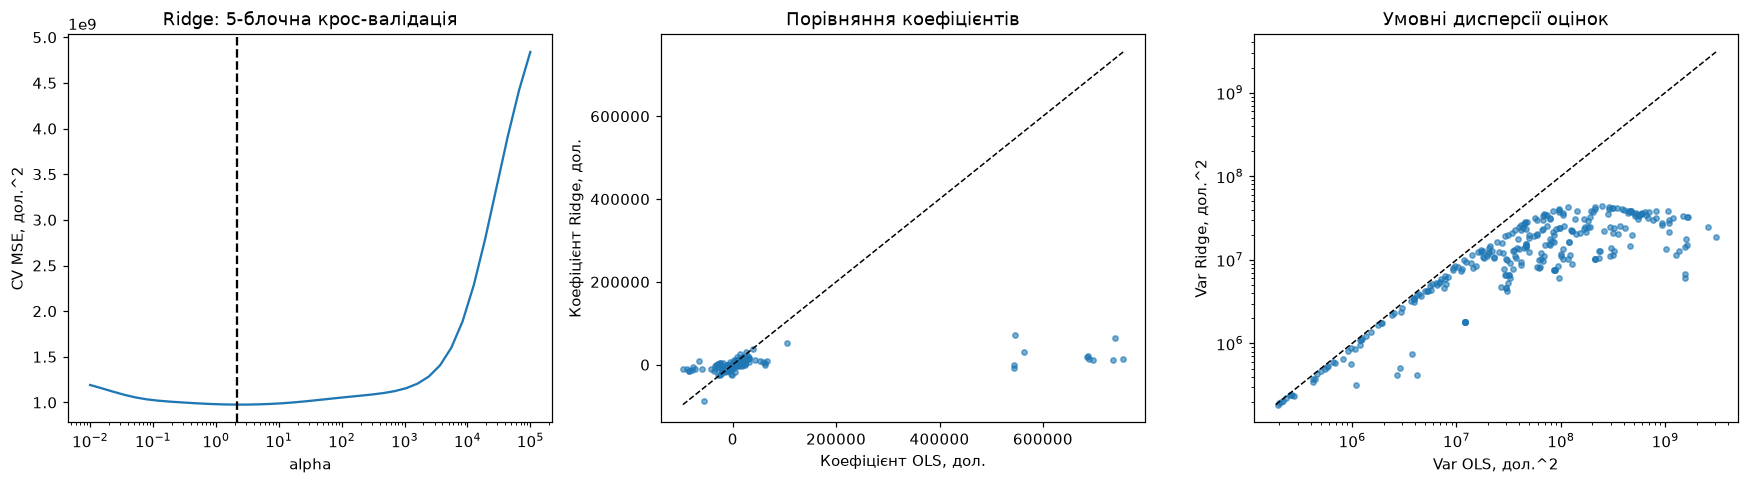
\includegraphics[width=1\linewidth,height=0.85\textheight,keepaspectratio]{../../figures/part1_ridge_ols.png}
\caption{Крос-валідація Ridge, коефіцієнти та умовні дисперсії.}
\end{figure}

\answerheading
Очікування до обчислень: додатний штраф Ridge зменшить умовні дисперсії
оцінок, але внесе зміщення. Менша дисперсія не гарантує меншої помилки
прогнозу на нових даних.

Обидві моделі оцінюємо на тих самих підготовлених ознаках. Ранг
центрованої матриці становить 280 за 294 ознак, тому коефіцієнти МНК не
єдині. Порівнюємо Ridge з розв'язком МНК, який повертає
\texttt{LinearRegression}: серед розв'язків він має найменшу суму
квадратів коефіцієнтів. Для нього використовуємо псевдообернену матрицю,
яка працює і за залежних стовпців.

Фіксуємо матрицю ознак і вибраний штраф та припускаємо, що похибки
некорельовані й мають однакову дисперсію. Оцінки матриць коваріацій
коефіцієнтів мають вигляд
\[\widehat{\operatorname{Var}}(\widehat\beta_{OLS})=\widehat\sigma^2 Z^+(Z^+)^T,\qquad
\widehat{\operatorname{Var}}(\widehat\beta_R)=\widehat\sigma^2 A_RA_R^T,\qquad A_R=(Z^TZ+\alpha I)^{-1}Z^T.\]
Тут \(\widehat\beta_{OLS}\) і \(\widehat\beta_R\) є оцінками
коефіцієнтів МНК і Ridge, \(Z\) є центрованою матрицею ознак, а \(Z^+\)
її псевдооберненою матрицею. Матриця \(A_R\) перетворює центровані ціни
на оцінки Ridge, \(\alpha\) є силою штрафу, \(I\) одиничною матрицею,
\(T\) позначає транспонування, а \(-1\) обернення матриці. Оцінку
дисперсії похибок \(\widehat\sigma^2\) отримуємо, ділячи суму квадратів
залишків МНК на \(n-r-1\), де \(n\) є кількістю навчальних спостережень,
\(r\) рангом \(Z\), а одиниця враховує вільний член. Діагоналі матриць
дають дисперсії окремих коефіцієнтів у таблиці.

Результати після обчислень

Крос-валідація вибрала для Ridge \(\alpha\approx2.154\). Коефіцієнт
\texttt{LotArea} зменшився з 5463 до 4115 дол. на одне навчальне
стандартне відхилення площі. Сума умовних дисперсій зменшилася з
\(6.198\cdot10^{10}\) до \(4.795\cdot10^9\) дол.², як і очікували.
Зміщення коефіцієнтів окремо не оцінювали.

